\documentclass[../main.tex]{subfiles}

\begin{document}


This is a non-binding timeline for this PhD. It is accepted that this will likely change and only represents estimates given the current available information, the timeline is available in Gantt format in Figure \ref{fig:gantt}

In creating this time-line for the PhD several assumptions were made:
\begin{itemize}
    \item \textbf{Holiday Periods:} Two weeks of holiday have been accounted for during the summer and a two-week period over Christmas and New Year. This timeline does not account for additional holidays, which will be determined later.
    \item Front-Loaded Research: The research plan is front-loaded, with significant emphasis placed on the early stages of the project. This approach allows additional literature searching, coding, and experimental setup to be completed in advance, providing a solid foundation for later stages of research, the research questions of which are currently flexible. This strategy also ensures that any necessary adaptations can be made based on early findings, reducing the risk of major delays later in the project. 

        \item \textbf{Research Flexibility:} Significant breaks are scheduled between work on research questions to allow for adaptation or extension if research questions need to be adjusted. In addition, there is a dedicated period for each of the three research themes before beginning coding or experimental setups. This time is intended for further literature review, acknowledging the rapidly evolving nature of this field. Advancement of the literature are expected before the start of each research question period.
    \item \textbf{Undetermined Research Questions:} Two research questions have deliberately been left open. Depending on the findings of the first three research questions, new research opportunities or developments in the field may emerge that require investigation.
    \item \textbf{Publication goals:} The goal is to produce at least one publishable piece of work for each research question. The preferential publication venue is SIGIR, recognised as the highest-rated publication venue for this sub-domain, aside from broader higher impact journals such as ACL. This goal is deliberately ambitious, as until the research is complete, it is impossible to determine the merits of its findings.
    \item \textbf{Conference Scheduling:} SIGIR abstract submissions and conferences occur around the same time each year, which has been considered in the planning. Note that many RQs are concluded prior to the expected submission dates.

\end{itemize}

\subsection{Potential Threats}

A risk matrix of all potential threats is outlined in Table \ref{tab:risk_matrix}.

\begin{itemize}
    \item \textbf{Research Delays:} Unforeseen challenges in research or coding could lead to delays. These could arise from the complexity of the research questions, issues with experimental setups, or unexpected results that require additional analysis. This is mitigated through periods at the end of research questions which can be utilised, if necessary.
    \item \textbf{Technological advancement:} The fast-moving nature of the field could result in the emergence of new technologies or methodologies that could make parts of the planned research less relevant or require a significant change of focus. This is mitigated through periods allowing additional literature review before coding on that research question.
    \item \textbf{Publication risks:} There is always the risk that the research might not yield results suitable for publication or that the publication process itself might be more time-consuming than anticipated, especially if revisions are required. The nature of the publication system is that there will be extended gaps between the completion of the research and its publication, making modification of the research to match a reviewer's expectations difficult.
    \item \textbf{Personal and Health Factors:} Extended periods of high-intensity work can lead to burnout or health problems, potentially affecting the planned schedule. The Gantt chart does not and cannot fully account for extended absences due to illness or other personal factors.
    \item \textbf{Open ended research questions:} It could be that at the time of reaching the open-ended research questions, a research area has not been identified. The author believes that this is unlikely, given that this field is limited, and other potential research questions have been dropped to ensure this flexibility.
    \item \textbf{Competing time constraints from PGDip:} Due to the concurrent requirements of the PGDip with this PHd, there will at times be constraints placed on my available time. So far, I believe, I have demonstrated good time keeping skills, and believe this schedule to be reasonable given the other competing time constraints. If there is a clash, PH.d. will take priority over PGDip.
\end{itemize}
\begin{landscape}
\begin{figure}
\centering
        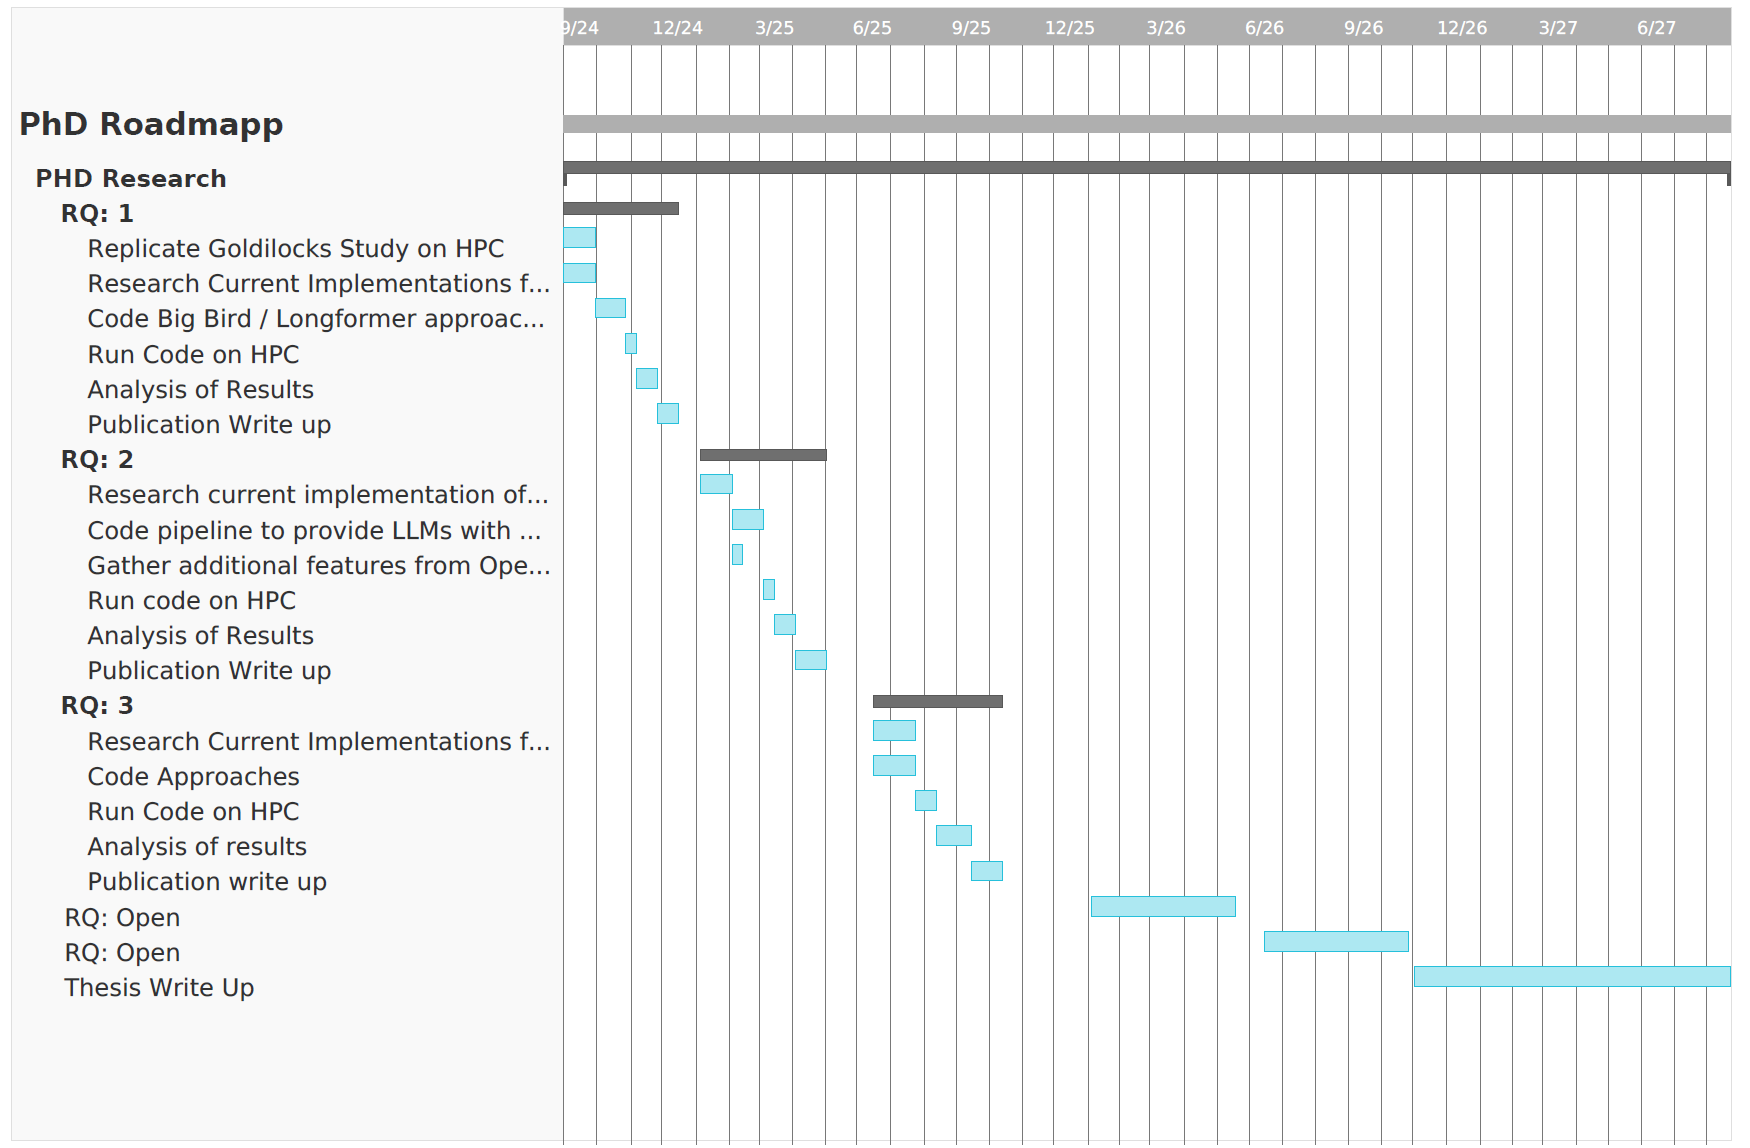
\includegraphics[width=1\linewidth]{sections//images/Gantt1.png}
        \caption{Gantt Chart for OVerview of Timeline for PHd}
        \label{fig:gantt}
    \end{figure}
\end{landscape}
    

\begin{landscape}
\begin{table}[t]
\centering
\footnotesize
\begin{tabular}{|c|c|c|c|>{\raggedright\arraybackslash}p{10cm}|}
\hline
\textbf{Threat} & \textbf{Likelihood (L)} & \textbf{Impact (I)} & \textbf{Risk} & \textbf{Response} \\
\hline
Research Delays & 3 & 4 & 12 & Reduce the number of research questions to mitigate delays. \\
\hline
Technological Advancement & 3 & 3 & 9 & Increase time allocated for additional literature review to stay updated with advancements. \\
\hline
Publication Risks & 3 & 3 & 9 & If results are not deemed valid during the analysis phase, proceed to the next research question without spending time on write-up. \\
\hline
Personal and Health Factors & 2 & 4& 8  & Prioritise health by taking regular breaks and managing workload effectively to avoid burnout. \\
\hline
Open-ended Research Questions & 2 & 3 & 6 & Continuously monitor new publications within the domain to ensure relevant and timely research questions. \\
\hline
Competing Time Constraints (PGDip) & 3 & 3 & 9 & Minimize involvement in PGDip activities where possible to focus on PhD work. \\
\hline
\end{tabular}
\caption{Risk Scoring Matrix for threats to PhD. Responses are provided for medium impact risks.}
\label{tab:risk_matrix}
\end{table}
\end{landscape}


\end{document}
